% !TEX root = ../OT4ML.tex

%%%%%%%%%%%%%%%%%%%%%%%%%%%%%%%%%%%%%%%%%%%%%%%%%%%%%%%%%%%%%%%%%%%%%%%%%%%
%%%%%%%%%%%%%%%%%%%%%%%%%%%%%%%%%%%%%%%%%%%%%%%%%%%%%%%%%%%%%%%%%%%%%%%%%%%
%%%%%%%%%%%%%%%%%%%%%%%%%%%%%%%%%%%%%%%%%%%%%%%%%%%%%%%%%%%%%%%%%%%%%%%%%%%
\section{Optimal Matching between Point Clouds}
\label{sec-matching}

This opening section isolates the simplest form of optimal transport: pairing two finite point clouds. The stakes are algorithmic and geometric at once: one sees the combinatorial nature of transport, the special simplicity of the line, and the first hints that convex relaxation will be necessary in higher dimension. Classical assignment algorithms such as the Hungarian method and auction methods~\cite{Kuhn1955,bertsekas1992auction} provide the computational backdrop, while the geometric examples prepare the Kantorovich relaxation.

%%%%%%%%%%%%%%%%%%%%%%%%%%%%%%%%%%%%%%%%%%%%%%%%%%%%%%%%%%%%%%%%%%%%%%%%%%%
\subsection{Monge Problem for Discrete Points}
\label{sec-monge-pbm}

This subsection formulates matching as Monge's deterministic transport problem on two equally weighted clouds. The one-dimensional case is a transparent reference case where the optimal map can be read off by sorting.

%%%%%%%
\paragraph{Matching Problem}


Given a cost matrix $(\C_{i,j})_{i \in \range{n}, j \in \range{m}}$ and assuming $n=m$, the optimal assignment problem aims to find a bijection $\sigma$ within the set $\Perm(n)$ of permutations of $n$ elements that solves
\eql{\label{eq-optimal-assignment}
	\umin{\sigma \in \Perm(n)} \frac{1}{n}\sum_{i=1}^n \C_{i,\sigma(i)}.
}
One could naively evaluate the cost function above using all permutations in the set $\Perm(n)$. However, this set has size $n!$, which becomes enormous even for small values of $n$.
%
In general, the optimal $\sigma$ is not unique.

\paragraph{1D Case}

In 1D, for convex cost, the matching defines a monotonic map.

\begin{proposition}[Monotone matching on the line]\label{prop-matching-1d-monotone}
Assume that the points $(x_i)_i$ and $(y_j)_j$ are pairwise distinct. If the cost is of the form $\C_{i,j}=h(x_i-y_j)$, where $h: \RR \rightarrow \RR^+$ is strictly convex (for example, $\C_{i,j}=|x_i-y_j|^p$ for $p > 1$), then any optimal $\sigma$ defines a strictly increasing map $x_i \mapsto y_{\sigma(i)}$ (and thus is unique), i.e.,
\eq{
	\forall (i,i'), \quad (x_i-x_{i'})(y_{\sigma(i)}-y_{\sigma(i')}) > 0.
}
\end{proposition}
\begin{proof}
Indeed, if this property is violated, i.e., there exists $(i,i')$ such that $(x_i-x_{i'})(y_{\sigma(i)}-y_{\sigma(i')}) < 0$, then one can define a permutation $\tilde{\sigma}$ by swapping the match, i.e., $\tilde{\sigma}(i)=\sigma(i')$ and $\tilde{\sigma}(i')=\sigma(i)$, yielding a strictly better cost, as proved in the following fact.
%
Let $h:\RR\to\RR$ be strictly convex and let $x < x'$ and $y < y'$. Then
\[
  h(x-y)+h(x'-y') < h(x-y')+h(x'-y).
\]
We set the gap $d:=y'-y > 0$ and define for every $s\in\RR$
\[
	  D(s):=\frac{h(s)-h(s-d)}{d}
	\quad\text{and}\quad
	\Delta:=h(x-y')+h(x'-y)-h(x-y)-h(x'-y') = d ( D(x'-y)-D(x-y) ).
\]
Because $h$ is strictly convex, $D$ is strictly increasing.
Since $x-y < x'-y$, monotonicity yields $D(x-y) < D(x'-y)$, that is $\Delta > 0$.
\end{proof}

This property extends by continuity to convex (not strictly convex) costs such as $|x-y|$, but in this case, the matching is not necessarily unique.
Note that if $h$ is concave instead of being convex, then the behavior is entirely different, and the optimal match tends to exchange the positions. In this case, there exists an $O(n^2)$ algorithm.

Therefore, the algorithm to compute an optimal transport is to sort the points, i.e., find some pair of permutations $\sigma_X, \sigma_Y$ such that
\eq{
	x_{\sigma_X(1)} \leq x_{\sigma_X(2)} \leq \ldots
	\qandq
	y_{\sigma_Y(1)} \leq y_{\sigma_Y(2)} \leq \ldots
}
and then an optimal match is mapping $x_{\sigma_X(k)} \mapsto y_{\sigma_Y(k)}$, i.e., an optimal transport is $\sigma = \sigma_Y \circ \sigma_X^{-1}$. The total computational cost is thus $O(n\log(n))$, using, for instance, the quicksort algorithm.

\begin{figure}[ht]
\centering
\begin{tabular}{@{}cc@{}}
\small two mixtures & \small one mode to three modes \\[-.15em]
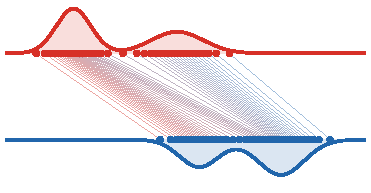
\includegraphics[width=.46\linewidth]{figures/matching-1d-quantile-assignment/quantile-assignment.pdf} &
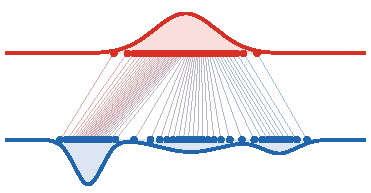
\includegraphics[width=.46\linewidth]{figures/matching-1d-quantile-assignment/central-to-three-modes.pdf}
\end{tabular}
\caption{One-dimensional optimal matching by quantile sorting. The red and blue curves are smooth laws used to generate equal-weight empirical measures; the dots are inverse-CDF samples at common quantile levels. The monotone assignment connects equal ranks, both for two Gaussian mixtures and for the transport from one central Gaussian toward a three-mode target law.}
\label{fig:matching-1d-quantile-assignment}
\end{figure}

%
Note that if $\phi : \RR \rightarrow \RR$ is an increasing map, one can apply this technique to costs of the form $h(|\phi(x)-\phi(y)|)$ with a change of variable.
%
A typical application is grayscale histogram equalization. The empirical cumulative distribution of the luminance values of an image is transported to a prescribed target histogram, often a uniform or reference-image histogram. In one dimension, the monotone rearrangement above gives the exact transport map, so the operation is both computationally simple and geometrically faithful: it matches distributions of intensities rather than individual pixels.

\begin{figure}[H]
\centering
\begin{tabular}{@{}cccc@{}}
\small $t=0$ & \small $t=1/3$ & \small $t=2/3$ & \small $t=1$ \\[-.15em]

\includegraphics[width=.21\linewidth]{figures/monge-histogram-equalization/image-t000.pdf} &

\includegraphics[width=.21\linewidth]{figures/monge-histogram-equalization/image-t033.pdf} &

\includegraphics[width=.21\linewidth]{figures/monge-histogram-equalization/image-t067.pdf} &

\includegraphics[width=.21\linewidth]{figures/monge-histogram-equalization/image-t100.pdf} \\[-.1em]
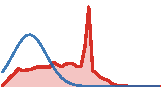
\includegraphics[width=.21\linewidth]{figures/monge-histogram-equalization/hist-t000.pdf} &

\includegraphics[width=.21\linewidth]{figures/monge-histogram-equalization/hist-t033.pdf} &

\includegraphics[width=.21\linewidth]{figures/monge-histogram-equalization/hist-t067.pdf} &

\includegraphics[width=.21\linewidth]{figures/monge-histogram-equalization/hist-t100.pdf}
\end{tabular}
\caption{Histogram equalization as one-dimensional Monge transport on pixel intensities. The map is the monotone rearrangement $T=Q_\beta\circ F_\alpha$, using the cumulative and quantile functions defined later in Definition~\ref{def-cdf-quantile}. The images are interpolated pointwise by $I_t=(1-t)I+tT(I)$, and the histograms show the empirical laws of these interpolated intensities; they are not binwise linear interpolations of histograms. This is the one-dimensional version of McCann displacement interpolation, discussed in Section~\ref{sec-monge-interpolation}.}
\label{fig:monge-histogram-equalization}
\end{figure}

Note that if $h$ is strictly convex, then all optimal assignments are increasing, and if the points are all distinct, this increasing map is unique. If $h$ is not strictly convex, for instance $c(x,y)=|x-y|$, non-increasing optimal assignments can also exist. This happens, for example, in the book-shifting problem with overlapping uniform distributions, where the mass in the intersection can stay fixed.

This efficient strategy to compute the OT in 1-D does not extend to higher dimensions. In 2-D, as already noted by Monge, one has the following property.

\begin{proposition}[Non-crossing optimal matchings]
	In dimension 2, for $c(x,y) = \norm{x-y}$, if $\sigma$ is an optimal assignment, then segments $[x_i,y_{\sigma(i)}]$ cannot cross.
\end{proposition}

\begin{proof}
	If two segments $[x_i,y_{\sigma(i)}]$ and $[x_j,y_{\sigma(j)}]$ cross at an interior point $z$, then the triangle inequality gives
	\[
		\norm{x_i-y_{\sigma(j)}}+\norm{x_j-y_{\sigma(i)}}
		<
		\norm{x_i-y_{\sigma(i)}}+\norm{x_j-y_{\sigma(j)}}.
	\]
	The assignment obtained by swapping $(\sigma(i),\sigma(j))$ therefore has a strictly smaller cost, which contradicts optimality.
\end{proof}

This property alone is, however, not enough to lead to an efficient algorithm. Non-crossing is only a necessary local test, not a compact certificate of optimality. For instance, if $n$ sources and $n$ targets are placed alternately on the boundary of a convex polygon, the number of non-crossing perfect matchings is the Catalan number
\[
	C_n=\frac{1}{n+1}\binom{2n}{n}\sim \frac{4^n}{\sqrt{\pi}n^{3/2}}.
\]
Thus even after forbidding crossings, an exhaustive search remains exponential. The two-segment swap in the proof above is nevertheless useful: it explains why a crossing matching cannot be optimal, but it does not select among the exponentially many planar matchings that survive this local test.

\begin{figure}[ht]
\centering
\begin{tabular}{ccc}
\small $c(x,y)=\norm{x-y}$ &
\small $c(x,y)=\norm{x-y}^2$ &
\small $c(x,y)=\norm{x-y}^6$ \\[-.15em]

\includegraphics[width=.30\linewidth]{figures/matching-2d-cost-exponent/p1.pdf} &

\includegraphics[width=.30\linewidth]{figures/matching-2d-cost-exponent/p2.pdf} &

\includegraphics[width=.30\linewidth]{figures/matching-2d-cost-exponent/p6.pdf}
\end{tabular}
\caption{Optimal assignments between the same two point clouds for three powers of the Euclidean distance. The source is a compact central Gaussian cloud and the target is a three-mode Gaussian mixture; this canonical geometry is reused in later coupling and regularization figures. The feasible set is unchanged, but increasing $p$ penalizes the longest edges more strongly and changes the global organization of the permutation.}
\label{fig:matching-2d-cost-exponent}
\end{figure}

The strict assignment model is also tied to equal cardinalities and equal weights. As soon as the target resolution changes or the weights are not uniform, a permutation no longer describes the feasible transports. One instead needs a nonnegative transport matrix with prescribed row and column sums, as illustrated in Figure~\ref{fig:matching-resolution-and-weights}; this is the finite-dimensional Kantorovich relaxation developed in Section~\ref{sec-kantorovich}.

\begin{figure}[ht]
\centering
\begin{tabular}{ccc}
\small balanced assignment &
\small coarser target &
\small nonuniform $\beta$ \\[-.15em]

\includegraphics[width=.30\linewidth]{figures/matching-resolution-and-weights/balanced.pdf} &
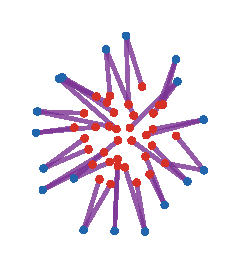
\includegraphics[width=.30\linewidth]{figures/matching-resolution-and-weights/rectangular.pdf} &

\includegraphics[width=.30\linewidth]{figures/matching-resolution-and-weights/weighted.pdf}
\end{tabular}
\caption{From assignments to transport plans, using the same central-source and three-mode-target geometry as Figure~\ref{fig:matching-2d-cost-exponent}. In the balanced equal-weight case, each source atom is matched to one target atom. With a coarser target or nonuniform target weights, the coupling matrix can merge or split mass; segment thickness and opacity encode its nonzero entries, and target marker areas encode the prescribed target masses.}
\label{fig:matching-resolution-and-weights}
\end{figure}


%%%%%%%%%%%%%%%%%%%%%%%%%%%%%%%%%%%%%%%%%%%%%%%%%%%%%%%%%%%%%%%%%%%%%%%%%%%
\subsection{Matching Algorithms}

This subsection briefly locates matching within classical combinatorial optimization. Its main point is that efficient algorithms exist, but their cleanest analysis is obtained only after introducing the linear-programming viewpoint.

Efficient algorithms exist to solve the optimal matching problem. The most well-known are the Hungarian method and auction algorithms~\cite{Kuhn1955,bertsekas1981new,bertsekas1992auction}. Auction algorithms use prices on the target points: each source bids for the target with largest reduced profit, the target price is increased, and the process terminates when the $\epsilon$-complementary slackness conditions are satisfied. For integer costs, choosing $\epsilon<1/n$ gives an exact optimum after a finite number of bids~\cite{bertsekas1992auction}. Section~\ref{sec-auction-dual-ascent} revisits this algorithm after Kantorovich duality and explains why it is a dual price method, parallel in spirit to Sinkhorn scaling.

\paragraph{Hungarian primal-dual method.}

The Hungarian method is best understood as a certificate-building algorithm for the assignment linear program. It maintains a partial matching $M$ and dual prices $(u_i,v_j)$ satisfying
\[
	u_i+v_j\leq C_{i,j}\qquad\forall i,j.
\]
The equality graph $E(u,v)=\{(i,j):u_i+v_j=C_{i,j}\}$ contains the edges whose reduced cost is zero. The algorithm only augments $M$ along alternating paths made of equality edges. Starting from an unmatched source, it grows an alternating tree with source set $S$ and target set $T$. If the tree reaches an unmatched target, the matching is augmented along the path. If no such edge exists, the dual variables are shifted by the smallest slack
\[
	\delta=\min_{i\in S,\ j\notin T}\bigl(C_{i,j}-u_i-v_j\bigr),
	\qquad
	u_i\leftarrow u_i+\delta\ (i\in S),\qquad
	v_j\leftarrow v_j-\delta\ (j\in T).
\]
This update preserves all inequalities $u_i+v_j\leq C_{i,j}$, keeps the current alternating tree tight, and creates at least one new equality edge leaving $S$. Maintaining these slacks incrementally gives the standard $O(n^3)$ implementation for an $n\times n$ assignment problem.

\begin{prop}[Correctness and complexity of the Hungarian primal-dual method]\label{prop-hungarian-correct}
	Assume the Hungarian method terminates with a perfect matching $\sigma$ contained in the equality graph
	\[
		E(u,v)=\enscond{(i,j)}{u_i+v_j=C_{i,j}},
	\]
	where $(u,v)$ is dual feasible, i.e. $u_i+v_j\leq C_{i,j}$ for all $(i,j)$. Then $\sigma$ is an optimal assignment. Moreover, the usual Hungarian updates terminate after finitely many augmentations.
	With maintained slacks, the method uses $O(n^3)$ arithmetic operations.
\end{prop}

\begin{proof}
	For any permutation $\tau$, dual feasibility gives
	\[
		\sum_i C_{i,\tau(i)} \geq \sum_i (u_i+v_{\tau(i)})
		= \sum_i u_i+\sum_j v_j.
	\]
	This is the weak duality lower bound. If $\sigma$ is contained in the equality graph, then
	\[
		\sum_i C_{i,\sigma(i)}
		= \sum_i u_i+\sum_j v_j,
	\]
	so the primal cost of $\sigma$ reaches the dual lower bound and is optimal.

	It remains to justify finite termination and the complexity bound. At each successful augmentation, the matching cardinality increases by one, so there are at most $n$ augmentations. During one augmentation phase, the algorithm grows an alternating tree in the equality graph. If no augmenting path is available, the dual update uses the smallest slack of an edge leaving the current tree. For edges inside the tree, adding $\delta$ to source labels and subtracting $\delta$ from target labels preserves tightness; for edges from $S$ to $T^c$, the definition of $\delta$ preserves feasibility and makes at least one new edge tight; all other inequalities are unchanged or become looser. Thus the reachable sets strictly grow between two failed augmentation attempts, and they can grow at most $n$ times within one phase. If the current slacks $\min_{i\in S}(C_{i,j}-u_i-v_j)$ are updated when a source enters $S$, each tree expansion costs $O(n)$. A phase therefore costs $O(n^2)$, and the $n$ phases give $O(n^3)$ operations. Hence the method reaches a perfect optimal matching.
\end{proof}

\paragraph{Network-flow viewpoint and applications.}

Their derivation and analysis are greatly simplified by introducing the Kantorovich relaxation and its associated dual problem. The transportation simplex and network-flow viewpoints go back to Dantzig's transportation linear program and modern minimum-cost-flow algorithms~\cite{Dantzig51,bertsekas1988dual,Orlin1997}.
%
These finite matching and assignment ideas also underlie color transfer between images. Grayscale equalization is one-dimensional, but transferring a full color palette requires transporting empirical measures in a three-dimensional color space, for instance RGB or Lab. Early color-transfer methods use affine statistics or iterated one-dimensional projections~\cite{reinhard2001color,pitie2005n}; replacing these projections by a genuine three-dimensional OT coupling gives a more intrinsic way to match colors while preserving the geometry of the palette~\cite{rabin-ssvm-11}.
